\documentclass[12pt]{article}
\usepackage[a4paper, total={6in, 9in}]{geometry}
\usepackage{graphicx}
\graphicspath{ {./images/output/} }
\usepackage{caption}
\usepackage[english]{babel}
\usepackage{titling}
\usepackage{float}
\usepackage{amsmath}
\usepackage{minted}
\usepackage{multicol}
% \usepackage{makecell}
\usepackage{tabularx}
\usepackage{multirow}
\usepackage{adjustbox}
% \usepackage{array}
% \usepackage{setspace}
% \usepackage{placeins}
\setlength{\parindent}{0pt}

% \usepackage{lipsum}

\title{Determination of Modulation Index of FM Wave}
\author{}
\date{}

\pagenumbering{gobble}
\begin{document}
\vspace*{\fill}
\begin{center}

    \emph{Heaven's Light is Our Guide} \\
    \textbf{Rajshahi University of Engineering and Technology} \\

    \begin{figure}[H]
        \centering
        
\includegraphics[scale=.34]{images/RUET_logo.png}
        \label{fig:ruet_logo}
    \end{figure}
    \vspace{5mm}

    \textbf{Course Code}\\
    ECE 3208\\
    \vspace{3mm}
    \textbf{Course Title}\\
    Communication Engineering Sessional

    \vspace{5mm}
    \textbf{Experiment Date:} {January 21, 2025},\\
    \textbf{Submission Date:} {February 11, 2025}\\

    \vspace{5mm}
    \textbf{Lab Report 3: \\
        Determination of Modulation Index of FM Wave}

    \vspace{15mm}

    \begin{tabular}{c|c}
        \textbf{Submitted to} & \textbf{Submitted by} \\
        Dr. Md. Kamal Hosain  & Md. Tajim An Noor     \\
        Professor             & Roll: 2010025         \\
        Dept of ETE, RUET     &                       \\
    \end{tabular}

\end{center}
\vspace*{\fill}


\pagebreak

\tableofcontents

\pagebreak
\pagenumbering{arabic}
\maketitle

\section*{Theory}
\addcontentsline{toc}{section}{Theory}
Frequency Modulation (FM) encodes information by varying the instantaneous frequency of a carrier wave, making it more resistant to noise than Amplitude Modulation (AM).

The message signal:
\[
    m(t) = A_m \cos(2 \pi f_m t)
\]

The carrier signal:
\[
    c(t) = A_c \cos(2 \pi f_c t)
\]

The FM modulated signal:
\[
    s(t) = A_c \cos\left(2 \pi f_c t + \beta \sin(2 \pi f_m t)\right)
\]
where \( \beta = \frac{\Delta f}{f_m} \).

The demodulated signal:
\[
    V_{\text{0}}(t) = \frac{f_{\text{inst}}(t) - f_c}{\Delta f}
\]

To determine \( \Delta f \):
\begin{enumerate}
    \item Observe the modulated signal on an oscilloscope.
    \item Measure the maximum (\( f_{\text{max}} \)) and minimum (\( f_{\text{min}} \)) frequencies.
    \item Calculate \( \Delta f = \frac{f_{\text{max}} - f_{\text{min}}}{2} \).
\end{enumerate}

The bandwidth (\( B \)) of an FM signal, according to Carson's rule:
\[
    B \approx 2 (\Delta f + f_m) = 2 f_m (\beta + 1)
\]

FM is widely used in radio broadcasting and two-way radio communication due to its noise immunity and efficient bandwidth use \cite{haykin2008communication, proakis2007digital}.

\section*{Required Apparatus}
\addcontentsline{toc}{section}{Required Apparatus}
\begin{itemize}
    \item ANALOGUE SIGNAL TRANSMISSION DL 3155M60
    \item Oscilloscope
    \item Connecting Wires
    \item Power Supply
\end{itemize}

\section*{Block Diagram}
\addcontentsline{toc}{section}{Block Diagram}
\subsection*{FM Modulation and Demodulation}
\begin{figure}[H]
    \centering
    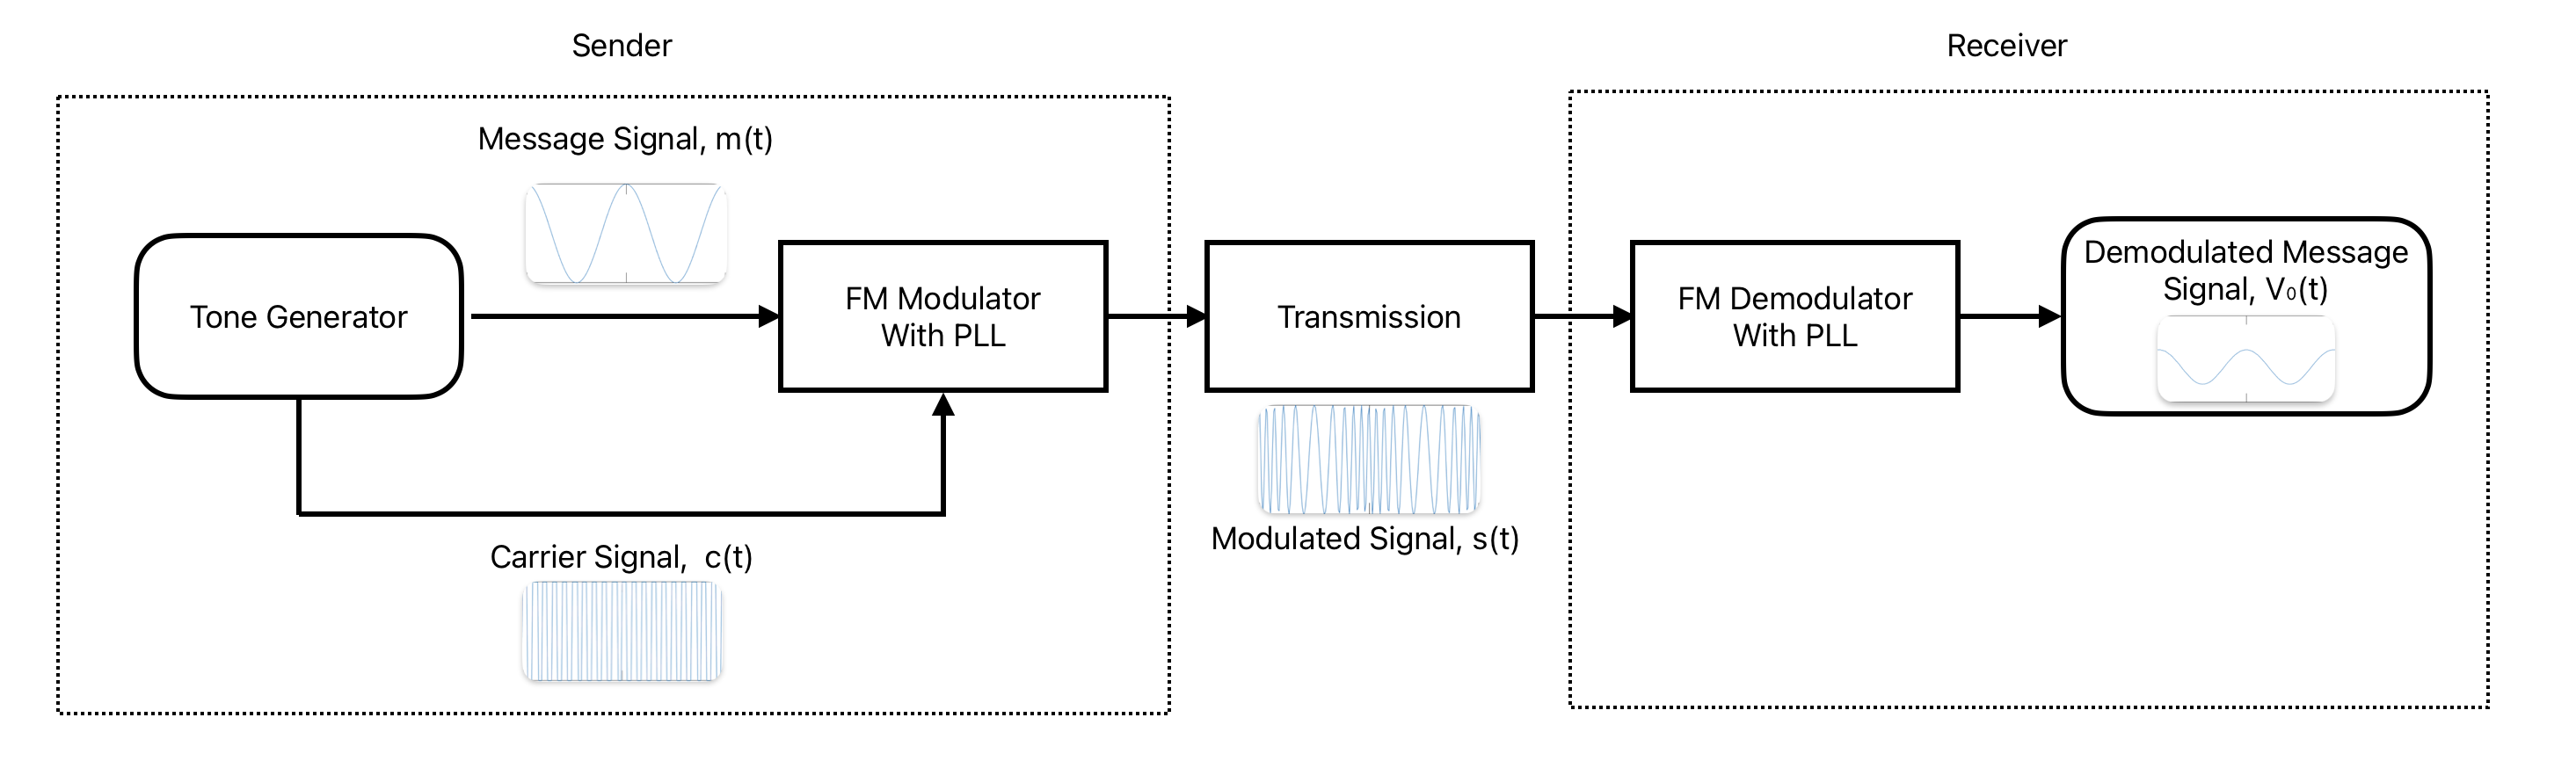
\includegraphics[width=\textwidth]{block.png}
    \caption{Block Diagram of FM Modulation and Demodulation}
    \label{fig:fm}
\end{figure}

\section*{Procedure}
\addcontentsline{toc}{section}{Procedure}
\begin{enumerate}
    \item The FM modulator and demodulator were connected as shown in the block diagram.
    \item The message signal was applied to the modulator and the modulated signal was observed on the oscilloscope.
    \item The frequency deviation and the modulating frequency were measured from the oscilloscope.
    \item The modulation index was calculated using the measured values.
    \item The experiment was repeated with different message signals and modulation frequencies to observe their effects.
    \item The observed values of frequency deviation, modulating frequency, and modulation index for each experiment were recorded.
\end{enumerate}


\section*{Experimental Data}
\begin{table}[H]
    \centering
    \begin{adjustbox}{width=\textwidth}
        \begin{tabular}{|c|c|c|c|c|c|c|}
            \hline
            \textbf{Reading no} & \multicolumn{2}{|c|}{\textbf{Message Signal's}} & \multicolumn{2}{|c|}{\textbf{Modulated Signal's Minimum}} & \multicolumn{2}{|c|}{\textbf{Modulated Signal's Maximum}}                                                                \\
            \cline{2-7}
                                & Time Period, (s)                                & Frequency, (kHz)                                          & Time Period, (s)                                          & Frequency, (kHz) & Time Period, (s)       & Frequency, (kHz) \\
            \hline
            1                   & \(1.4 \times 10^{-4}\)                          & 7.142                                                     & \(1.1 \times 10^{-5}\)                                    & 90.90            & \(3 \times 10^{-5}\)   & 33.33            \\
            \hline
            2                   & \(1.4 \times 10^{-4}\)                          & 7.142                                                     & \(1.05 \times 10^{-5}\)                                   & 95.24            & \(3.3 \times 10^{-5}\) & 30.3             \\
            \hline
            3                   & \(9 \times 10^{-5}\)                            & 11.11                                                     & \(1.2 \times 10^{-5}\)                                    & 83.33            & \(2.5 \times 10^{-5}\) & 40               \\
            \hline
            4                   & \(2.4 \times 10^{-4}\)                          & 3.937                                                     & \(1.1 \times 10^{-5}\)                                    & 90.91            & \(2.4 \times 10^{-5}\) & 41.67            \\
            \hline
        \end{tabular}
    \end{adjustbox}
\end{table}

\section*{Calculations}
\addcontentsline{toc}{section}{Calculations}
The modulation index (\( \beta \)) is calculated using the formula:

\[
    \beta = \frac{\Delta f}{f_m}
\]
where \( \Delta f \) is the frequency deviation and \( f_m \) is the frequency of the message signal.

The bandwidth (\( B \)) of an FM signal can be calculated using Carson's rule:
\[
    B \approx 2 (\Delta f + f_m) = 2 f_m (\beta + 1)
\]

\begin{enumerate}
    \item For Reading 1:
          \[
              f_m = 7.142 \text{ kHz}
          \]
          \[
              \Delta f = \frac{90.90 - 33.33}{2} \text{ kHz} = 28.785 \text{ kHz}
          \]
          \[
              \beta = \frac{28.785}{7.142} \approx 4.03
          \]
          \[
              B \approx 2 \times 7.142 \text{ kHz} \times (4.03 + 1) \approx 71.42 \text{ kHz}
          \]

    \item For Reading 2:
          \[
              f_m = 7.142 \text{ kHz}
          \]
          \[
              \Delta f = \frac{95.24 - 30.3}{2} \text{ kHz} = 32.47 \text{ kHz}
          \]
          \[
              \beta = \frac{32.47}{7.142} \approx 4.55
          \]
          \[
              B \approx 2 \times 7.142 \text{ kHz} \times (4.55 + 1) \approx 81.42 \text{ kHz}
          \]

    \item For Reading 3:
          \[
              f_m = 11.11 \text{ kHz}
          \]
          \[
              \Delta f = \frac{83.33 - 40}{2} \text{ kHz} = 21.665 \text{ kHz}
          \]
          \[
              \beta = \frac{21.665}{11.11} \approx 1.95
          \]
          \[
              B \approx 2 \times 11.11 \text{ kHz} \times (1.95 + 1) \approx 67.11 \text{ kHz}
          \]

    \item For Reading 4:
          \[
              f_m = 3.937 \text{ kHz}
          \]
          \[
              \Delta f = \frac{90.91 - 41.67}{2} \text{ kHz} = 24.62 \text{ kHz}
          \]
          \[
              \beta = \frac{24.62}{3.937} \approx 6.25
          \]
          \[
              B \approx 2 \times 3.937 \text{ kHz} \times (6.25 + 1) \approx 63.50 \text{ kHz}
          \]
\end{enumerate}

\section*{Results}
\addcontentsline{toc}{section}{Results}
The modulation index (\( \beta \)) and bandwidth (\( B \)) for each reading are summarized as follows:
\begin{itemize}
    \item For Reading 1:
          \begin{itemize}
              \item Modulation Index: \( \beta \approx 4.03 \)
              \item Bandwidth: \( B \approx 71.42 \text{ kHz} \)
          \end{itemize}
    \item For Reading 2:
          \begin{itemize}
              \item Modulation Index: \( \beta \approx 4.55 \)
              \item Bandwidth: \( B \approx 81.42 \text{ kHz} \)
          \end{itemize}
    \item For Reading 3:
          \begin{itemize}
              \item Modulation Index: \( \beta \approx 1.95 \)
              \item Bandwidth: \( B \approx 67.11 \text{ kHz} \)
          \end{itemize}
    \item For Reading 4:
          \begin{itemize}
              \item Modulation Index: \( \beta \approx 6.25 \)
              \item Bandwidth: \( B \approx 63.50 \text{ kHz} \)
          \end{itemize}
\end{itemize}


\section*{Matlab Simulation}
\addcontentsline{toc}{section}{Matlab Simulation}

\subsection*{Code:}
\addcontentsline{toc}{subsection}{Code}

\inputminted[linenos,breaklines,breakanywhere]{matlab}{./assets/fm.m}

\section*{Output}
\addcontentsline{toc}{section}{Output}

\subsection*{Experimental Output}
\addcontentsline{toc}{subsection}{Experimental Output}
\begin{figure}[H]
    \centering
    \begin{minipage}{0.45\linewidth}
        \centering
        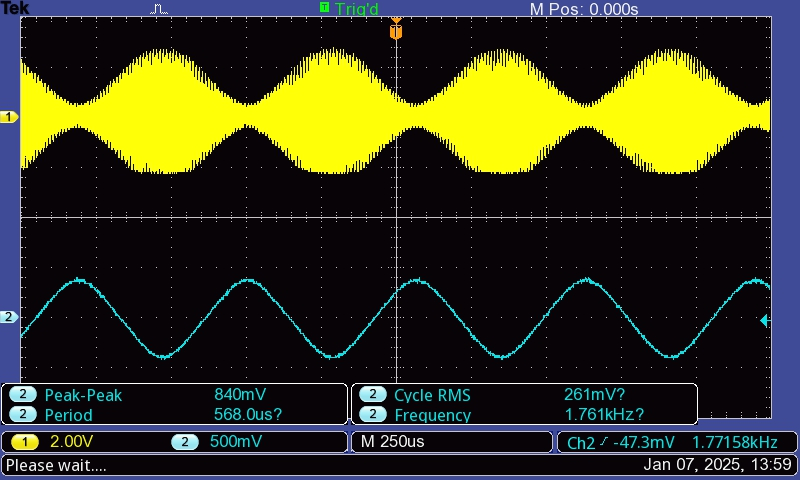
\includegraphics[width=\linewidth]{p1-undMod-msg.JPG}
        \caption{AM; Yellow: Under-modulated, Blue: Message}
        \label{fig:pic1}
    \end{minipage}
    \hfill
    \begin{minipage}{0.45\linewidth}
        \centering
        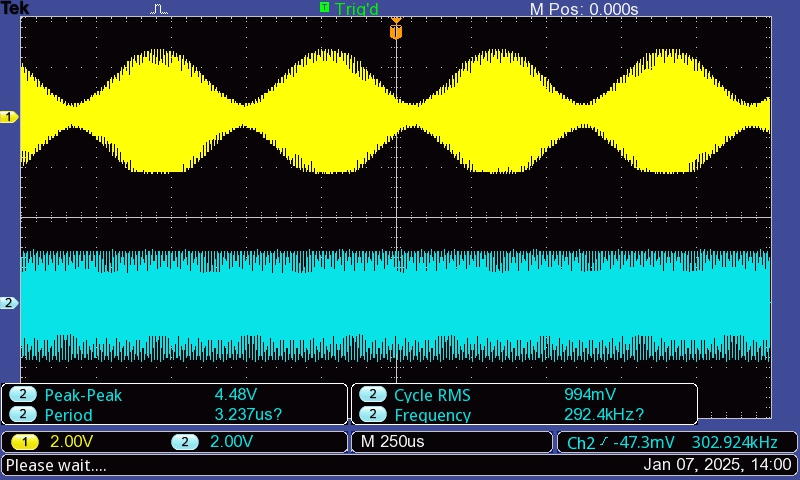
\includegraphics[width=\linewidth]{p2-undMod-car.JPG}
        \caption{AM; Yellow: Under-modulated, Blue: Carrier}
        \label{fig:pic2}
    \end{minipage}
    \vspace{1em}
    \begin{minipage}{0.45\linewidth}
        \centering
        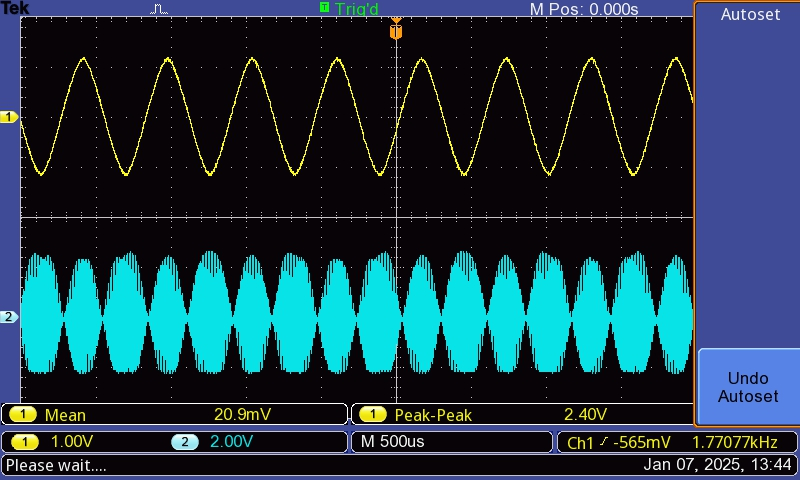
\includegraphics[width=\linewidth]{p3-msg-100mod.JPG}
        \caption{AM; Yellow: Message, Blue: 100\% Modulated}
        \label{fig:pic3}
    \end{minipage}
    \hfill
    \begin{minipage}{0.45\linewidth}
        \centering
        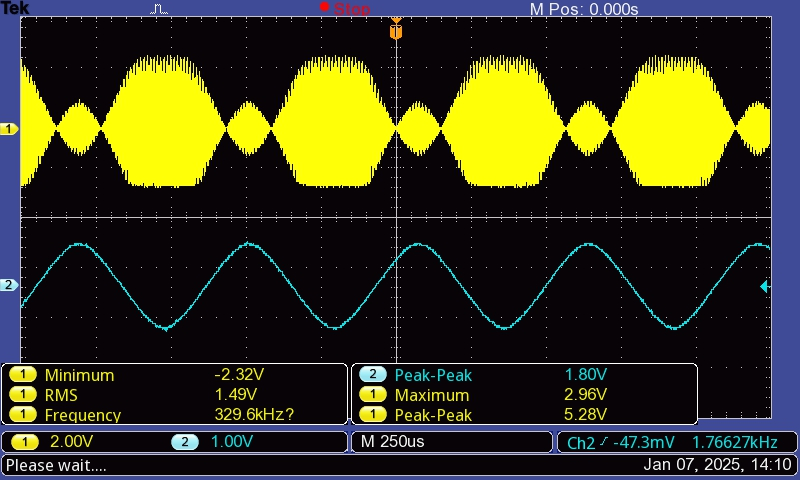
\includegraphics[width=\linewidth]{p4-ovMod-msg.JPG}
        \caption{AM; Yellow: Over-modulated, Blue: Message}
        \label{fig:pic4}
    \end{minipage}
    \vspace{1em}
    \begin{minipage}{0.45\linewidth}
        \centering
        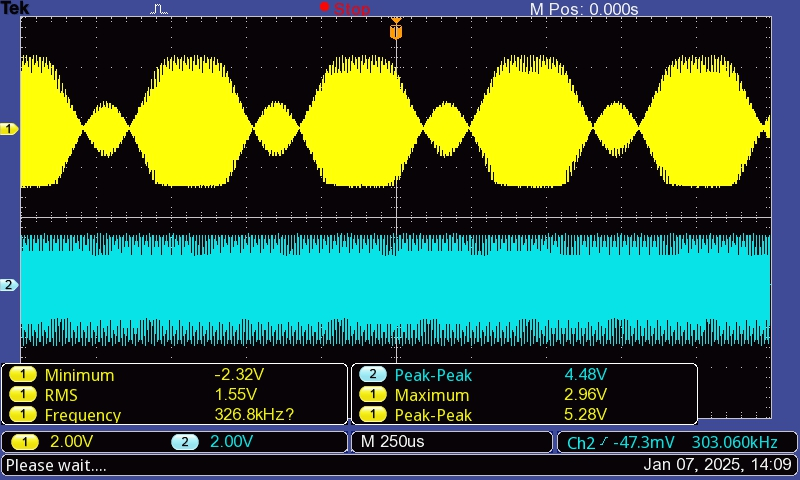
\includegraphics[width=\linewidth]{p5-ovMod-car.JPG}
        \caption{AM; Yellow: Over-modulated, Blue: Carrier}
        \label{fig:pic5}
    \end{minipage}
    \hfill
    \begin{minipage}{0.45\linewidth}
        \centering
        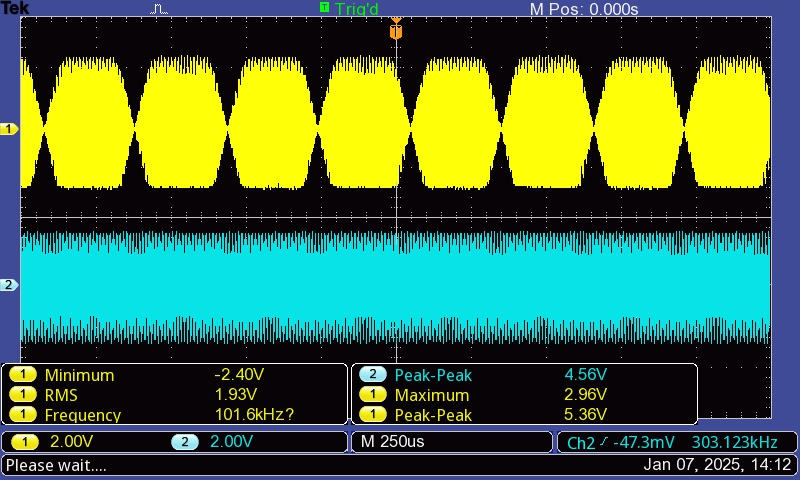
\includegraphics[width=\linewidth]{p6-dsb-mod-car.JPG}
        \caption{DSB\-SC; Yellow: Modulated, Blue: Carrier}
        \label{fig:pic6}
    \end{minipage}
\end{figure}

\pagebreak

\begin{figure}[H]
    \centering
    \begin{minipage}{0.45\linewidth}
        \centering
        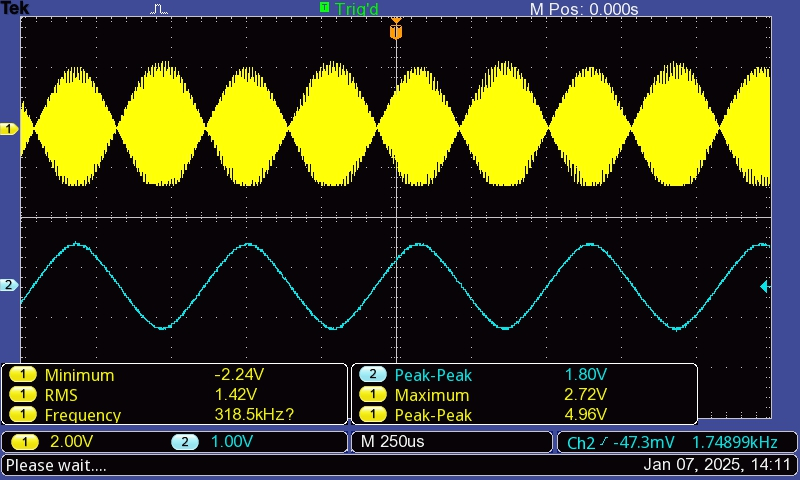
\includegraphics[width=\linewidth]{p7-dsb-mod-msg.JPG}
        \caption{DSB\-SC; Yellow: Modulated, Blue: Message 1}
        \label{fig:pic7}
    \end{minipage}
    \hfill
    \begin{minipage}{0.45\linewidth}
        \centering
        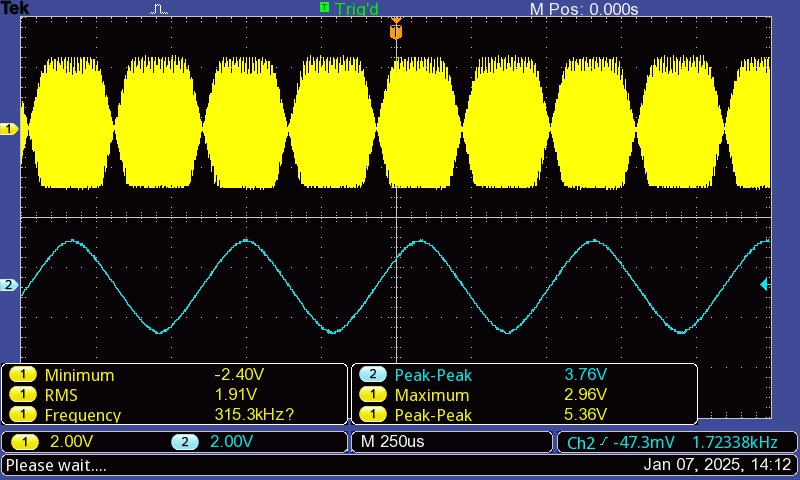
\includegraphics[width=\linewidth]{p8-dsb-mod-msg2.JPG}
        \caption{DSB\-SC; Yellow: Modulated, Blue: Message 2}
        \label{fig:pic8}
    \end{minipage}
    \vspace{1em}
    \begin{minipage}{\linewidth}
        \centering
        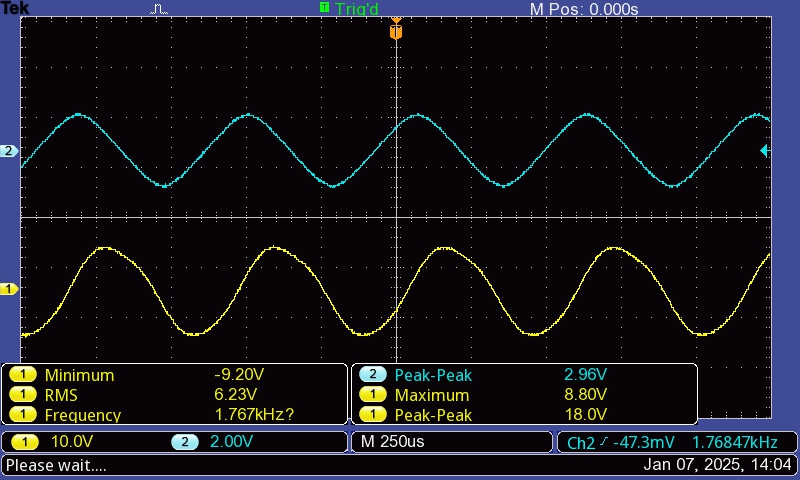
\includegraphics[width=0.4\linewidth]{p9-dsb-msg-Demod.JPG}
        \caption{DSB\-SC; Yellow: Message, Blue: Demodulated Message}
        \label{fig:pic9}
    \end{minipage}
\end{figure}

\subsection*{Matlab Simulation Output}
\addcontentsline{toc}{subsection}{Matlab Output}
\begin{figure}[H]
    \centering
    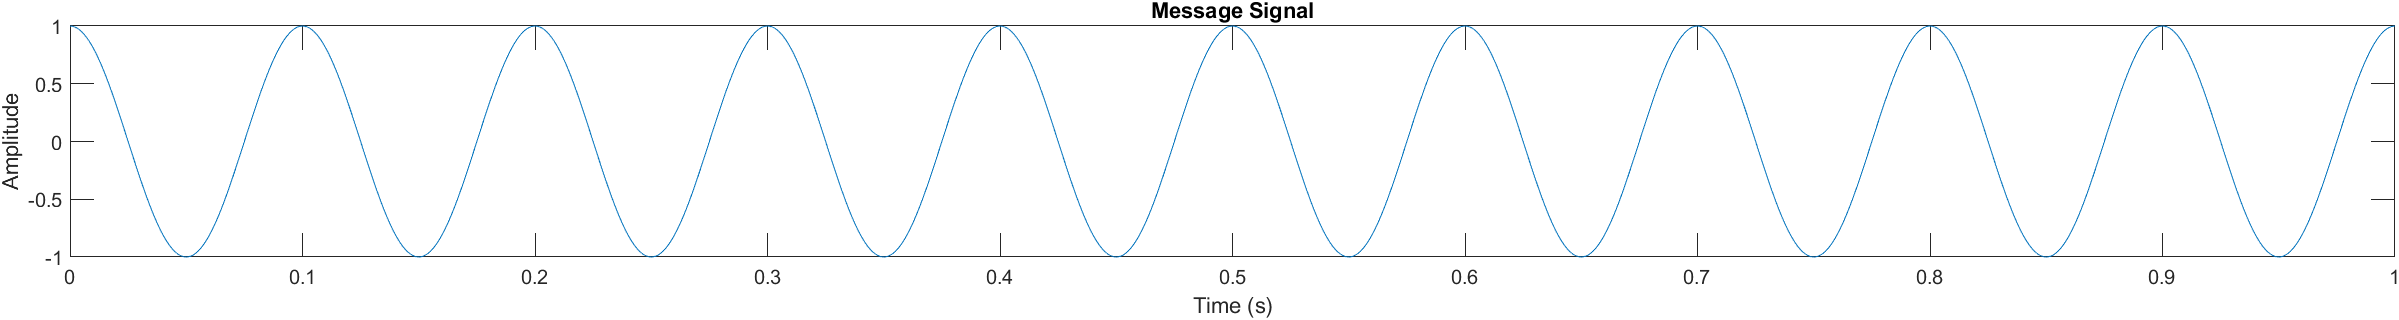
\includegraphics[width=\textwidth]{msg.png}
    \caption{Message Signal}
    \label{fig:img2}
\end{figure}

\begin{figure}[H]
    \centering
    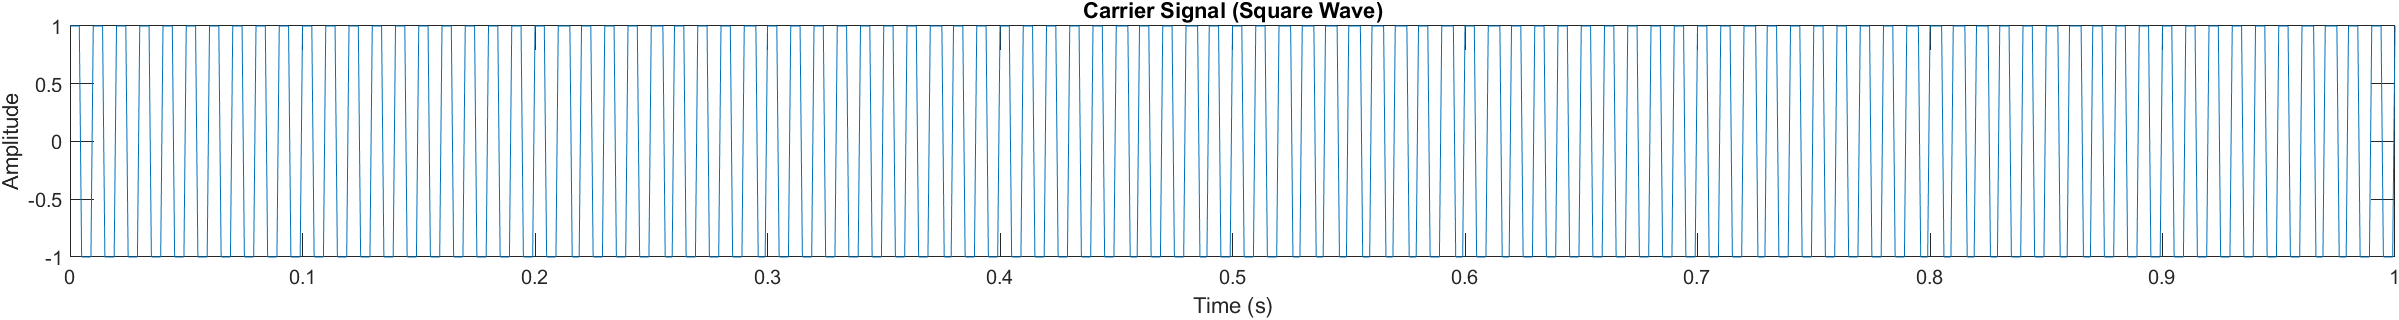
\includegraphics[width=\textwidth]{car.png}
    \caption{Carrier Signal, Square Wave}
    \label{fig:img11}
\end{figure}

\begin{figure}[H]
    \centering
    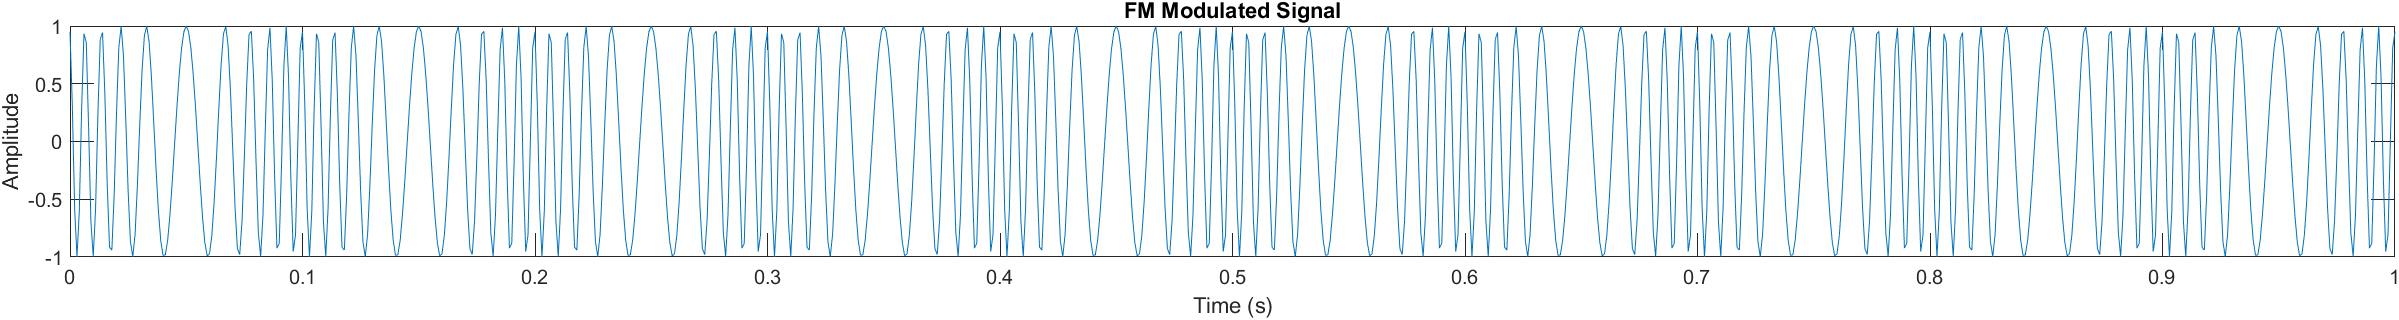
\includegraphics[width=\textwidth]{mod.png}
    \caption{FM Modulated Signal}
    \label{fig:img3}
\end{figure}

\begin{figure}[H]
    \centering
    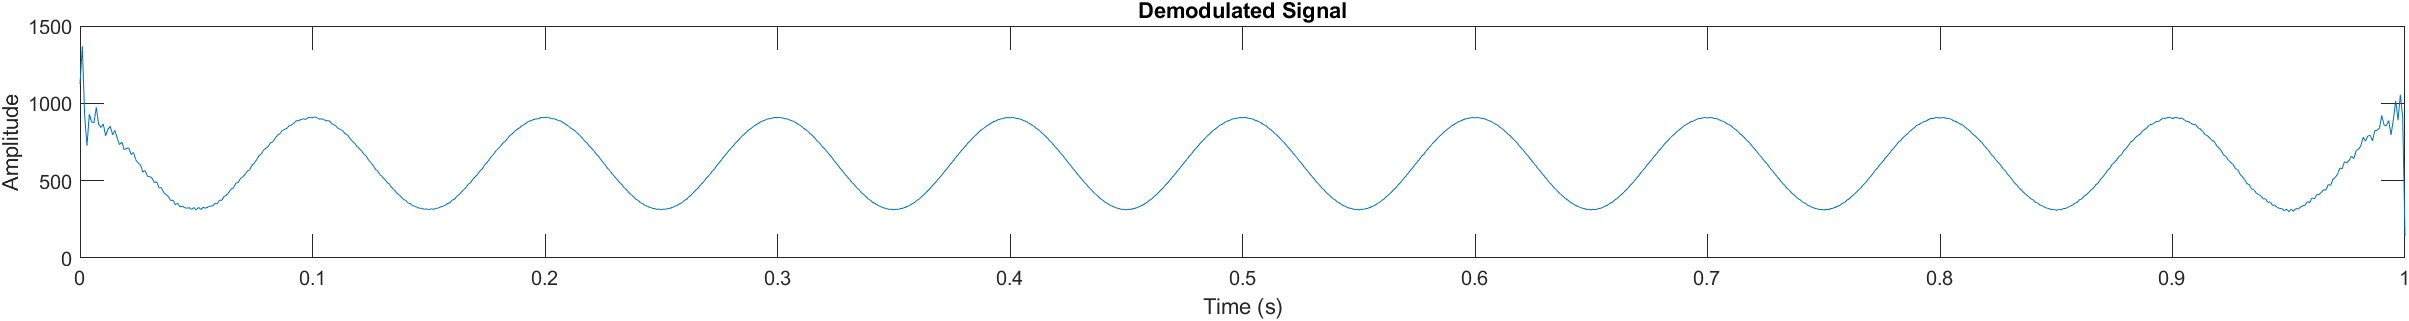
\includegraphics[width=\textwidth]{demod.png}
    \caption{Demodulated Signal}
    \label{fig:img4}
\end{figure}


\section*{Discussion and Conclusion}
\addcontentsline{toc}{section}{Discussion and Conclusion}
The modulation index (\( \beta \)) was found to be crucial in Frequency Modulation (FM) as it determined the bandwidth and the number of significant sidebands. In this experiment, \( \beta \) was calculated for different message signals and modulation frequencies using \( \beta = \frac{\Delta f}{f_m} \). Significant variations in \( \beta \) (1.95 to 6.25) were observed, impacting the bandwidth and quality of FM signals. The Matlab simulations confirmed the relationship between \( \beta \) and bandwidth, highlighting the importance of selecting an appropriate \( \beta \) for efficient communication. Valuable insights into the effects of \( \beta \) on FM signals and its significance in FM modulation were provided by this experiment.
\\\\
Matlab simulations confirmed the relationship between \( \beta \) and bandwidth, highlighting the importance of selecting an appropriate \( \beta \) for efficient communication. Valuable insights into the effects of \( \beta \) on FM signals and its significance in FM modulation were provided by this experiment. The results obtained from the experiment and Matlab simulations were consistent, demonstrating the accuracy and reliability of the calculations. Overall, the experiment was successful in determining the modulation index of FM waves and understanding its impact on signal quality and bandwidth.

\bibliographystyle{IEEEtran}
\renewcommand{\bibname}{References}
\addcontentsline{toc}{section}{References}
\bibliography{ref}

\end{document}
